\section{Charged fermions and the Fermion-Boson Correspondence}

\subsection{Representation}

Here I use the notation of~\cite{Dijkgraaf:2008ua, Justin2008} with
some small changes in~\cite{Alexandrov:2012tr, Marino:2005sj}. Other useful references
are \cite{Jimbo:1983if, Babelon2003, Borot2015}. The idea we want to
explore is the relation between Young diagrams and free fermions. We
start with the definition of the generating functions
\begin{equation}
 \psi(z) = \sum_{r \in \mathbb{Z} + 1/2} \psi_{-r} z^{r - 1/2}\qquad 
 \psi^\star(z) = \sum_{r \in \mathbb{Z} + 1/2} \psi_{r}^\star z^{r - 1/2}\; . 
\end{equation}
where the operators \(\psi_r\) and \(\psi_s^\ast\), satisfy the canonical
anticommutation relations
\begin{subequations}
\begin{equation}
\label{anticom}
\{\psi_r, \psi_s\} = \{\psi_r^\star, \psi_s^\star\} = 0
\qquad \{\psi_r, \psi_s^\star\} =\delta_{rs} \quad r, s \in \mathbb{Z}+1/2\; . 
\end{equation}
We can also define the occupancy and vacancy operators at the position
\(r\) 
\begin{equation}
\eta_r = \psi_r^\star \psi_r \, \quad
\zeta_r = 1- \psi_r^\star \psi_r\; .
\end{equation}
\end{subequations}
This is a simple model of charged free fermions, where the particles
are created by the operator \(\psi^\star_r\) and annihilated by
\(\psi_r\) at the \(r^{th}\) site. Equivalently, holes at the site
\(r\) are created by \(\psi_r\) and are annihilated by
\(\psi_r^\star\).

The vacuum configuration \(\ket{\bm{0}}\) is defined by the dirac Sea
filled up to the location \(r=0\), that is
\begin{center}
    \begin{tikzpicture}
    \node at (-4,0) { \(|\bm{0}\rangle=\)};
    \node at (-3,0) {\(\cdots\)};
    \draw (-2.5,0) -- (-2,0);
    \node at (-2,0) {\(\bullet\)};
    \draw (-2,0) -- (-1,0);
    \node at (-2,-.5) {\(-\tfrac{3}{2}\)};
    \node at (-1,0) {\(\bullet\)};
    \draw (-1,0) -- (-.06,0);
    \node at (-1,-.5) {\(-\tfrac{1}{2}\)};
    \node at (0,0) {\(\circ\)};
    \draw (.06,0) -- (.95,0);
    \node at (0,-.5) {\(\tfrac{1}{2}\)};
    \node at (1,0) {\(\circ\)};
    \draw (1.05,0) -- (1.5,0);
    \node at (1,-.5) {\(\tfrac{3}{2}\)};
    \node at (2,0) {\(\cdots\)};
  \end{tikzpicture}
\end{center}	
We assume that this state exists. Alternatively, one might define the empty state
\(\ket{\bm{\infty}}\) as \(\psi_r\ket{\bm{\infty}} = 0 \), \(\forall \ r \), therefore
\(\ket{\bm{0}} = \prod_{r < 0} \psi^\star_r \ket{\bm{\infty}}\). Regardless the case,
these definitions give equivalent results. 

We then have
\begin{equation}
\psi_{r}^\star\ket{\bm{0}}=0\ \ \ r< 0\; , \qquad  
\psi_{r} \ket{\bm{0}} = 0 \ \ \ r> 0
\end{equation}
The dual vacuum is defined as
\begin{equation}
\bra{\bm{0}} \psi_{r}=0\ \ \ r< 0\; , \qquad  
\bra{\bm{0}} \psi_{r}^\star = 0 \ \ \ r> 0\; ,
\end{equation}
therefore, we have the relation \((\psi_r)^\dagger\equiv \psi_r^\star\).

We can also build the shifted vacuum \(\ket{\ell}\) with \(\ell \in
\mathbb{Z}\) as
\begin{equation}
  \label{eq:charged-states}
  \ket{\ell} = 
  \left\{
  \begin{array}{ll}
    \psi^\star_{\ell - 1/2} \psi^\star_{\ell - 3/2} \cdots \psi^\star_{3/2} \psi^\star_{1/2} \ket{\bm{0}} & \ell > 0 \\
    \psi_{\ell + 1/2} \psi_{\ell + 3/2} \cdots \psi^\star_{-3/2} \psi^\star_{-1/2} \ket{\bm{0}} & \ell < 0
  \end{array}
  \right.
\end{equation}
These states satisfy
\begin{equation}
\psi_r\ket{\ell} = 0 \quad r > \ell \quad , \quad  
\psi_r^\star\ket{\ell} = 0  \quad r < \ell \; .
\end{equation}
Let us denote the Fock spaces labeled by these vacua as
\(\mathcal{F}_\ell\), for a complete discussion on the
structure of these spaces, see~\cite{Wheeler:2010vmq}. 
In particular, we have
\begin{equation}
\ket{\ell + 1} = \psi^\ast_{\ell + 1/2} \ket{\ell} \qquad
\ket{\ell} = \psi_{\ell + 1/2} \ket{\ell + 1} \; .
\end{equation}

Many of the results and identities we use have been explained in the
review~~\cite{Alexandrov:2012tr}. In order to pass from their notation
to ours, we can simply consider the transformation
\begin{equation}
\psi_k \equiv (\psi_{AZ})^\star_{k - 1/2} \qquad
\psi_k^\star \equiv (\psi_{AZ})_{k - 1/2} \; .
\end{equation}
where \textrm{AZ} stands for \emph{Alexandrov-Zabrodin.}

%%%%%%%%%%%%%%%%%%%%%%%%%%%%%%%%%%%%%%%%%%%%%%%%%%
%%%%%%%%%%%%%%%%%%%%%%%%%%%%%%%%%%%%%%%%%%%%%%%%%%

\subsection{States and Partitions}

A partition is a sequence of weakly decreasing non-negative integers,
\(\mu_i \geq \mu_{i+1}\) \(i = 1, \dots, n\). We can think of
partition as Young diagrams, where the \(i^{th}\) line has \(\mu_i\)
boxes. Given the partition \(\mu = (\mu_1, \mu_2, \dots, \mu_r)\),
the Frobenius coordinates \(\mu = (\alpha_j , \beta_j)\) are defined as
\begin{subequations}
\begin{equation}
\alpha_j=\mu_j - j \; , \quad 
\beta_j=\mu^T_j - j \; .
\end{equation}
It is convenient to write 
\begin{equation}
a_j=\alpha_j +\frac{1}{2}	\; , \quad 
b_j=\beta_j+\frac{1}{2}\; 
\end{equation}
and hereafter, these are the Frobenius coordinates we work with. For
further details, see~\cite{Alexandrov:2012tr}.
\end{subequations}
Moreover, we denote the number of
boxes in a partition \(\mu\) as
\begin{equation}
\#\texttt{Boxes}\equiv |\mu| = \sum_{j=1}^d (a_j+b_j)
\end{equation}

Given a partition \(\mu = (\mu_1, \mu_2, \cdots, \mu_n)\), one
can associate a fermionic state \cite{Dijkgraaf:2008ua, Okounkov:2003sp}
\begin{equation}
\label{eq:part-states}
\ket{\mu} = (-1)^{b(\lambda)} \prod_{j=1}^d \psi_{a_j}^\star \psi_{-b_j}\ket{\bm{0}}\; , \qquad
\langle \mu | = (-1)^{b(\lambda)}  \bra{\bm{0}}\prod_{j=1}^d  \psi_{-b_j}^\star \psi_{a_j}\;
,\quad a_j, b_j>0\ \ \forall j\; ,
\end{equation}
where we have added the factor \(b(\lambda) = \sum_{j = 1}^d (b_j -
1/2)\) for convenience. In~\cite{Alexandrov:2012tr}, the authors
define the same factor in the Schur polynomials expansion. We have
moved this factor to the states, as in~\cite{Marino:2005sj}, so that
the Schur polynomials expansio does not have any negative sign moving
around. It is worth noticing that if we have different partitions,
\(\ket{\lambda} \neq \ket{\nu}\), then there is a mismatch in the
number of pairs \(\psi^\star \psi\), and the states are orthonormal,
\(\langle \mu |\nu \rangle=\delta_{\mu\nu}\).

It is just a combinatorial exercice to show that the partition
states~\ref{eq:part-states}, and more generally the charged states,
can be equivalently written as
\begin{equation}
  \label{eq:part-states:2}
  \ket{\mu, \ell} = \psi^\star_{\ell + \mu_1 - 1/2} \dots
  \psi^\star_{\ell + \mu_n - n + 1/2} \ket{\ell - n}\; .
\end{equation}
See~\cite{Alexandrov:2012tr} for a discussion on both representations.

The normal ordering (with respect to the vacuum \(\ket{\bm{0}}\) is
defined as
\begin{equation}
:\psi_s \psi_r^\star: = \psi_s \psi_r^\star - \bra{\bm{0}} \psi_s
  \psi_r^\star \ket{\bm{0}} \; .
\end{equation}
That means that we need to move all creation operators to the left, and all
annihilation operators to the left, taking into account the negative factors
comming from the anticommutation relations. That is
\begin{equation}
:\psi_s \psi_r^\star:   = - :\psi_r^\star \psi_s: = 
\left\{
\begin{array}{rll}
-\psi_r^\star \psi_s && r>0 \\
\psi_s \psi_r^\star && r<0 
\end{array}	
\right.
\end{equation}

Using these relations, one can see that the number of boxes in
a generic partition \(\ket{\mu}\) is the eigenvalue of the following
operator \cite{Marino:2005sj}
\begin{equation}
L_0 = \sum_{r \in \mathbb{Z} + 1/2} r :\psi_{-r} \psi_r^\star:
\end{equation}
Therefore, we have
\begin{equation}
q^{L_0}|\mu \rangle = q^{|\mu|}|\mu \rangle \; .
\end{equation}	

% CHECK THESE THINGS LATER
% One interpretation to this system is given in terms of the free fermion
% \begin{subequations}
% \begin{equation}
% H= \sum_r r  \psi_r^\star \psi_r \; .
% \end{equation}
% It is easy to see that the state \(\ket{\bm{0}}\) is, indeed,
% a vacuum of the free Hamiltonian
% \begin{equation}
% H=\sum_r r :\psi^\star_r \psi_r: \; .
% \end{equation} 
% Explicitly, we have
% \begin{equation}
% \begin{split} 
%   H \ket{\bm{0}} & = \left(  \sum_{r<0} r  :\psi^\star_r \psi_r:  + \sum_{r>0} r 
%    :\psi^\star_r \psi_r:  \right) \ket{\bm{0}}  \\
%   & = \left(  \sum_{r<0} r  :\psi^\star_r \psi_r:  + \sum_{r>0} r  :\psi^\star_r 
%    \psi_r:  \right) \ket{\bm{0}}  \\
%   & = \left( - \sum_{r<0} r \psi_r \psi^\star_r  +
%        \sum_{r>0} r \psi^\star_r \psi_r \right) \ket{\bm{0}} = 0	
% \end{split}
% \end{equation}
% The Hamiltonian above is equivalent to the continuous system
% \begin{equation}
% S\sim \int d z\ \psi^\star(z) \partial \psi(z)\ \ \Rightarrow \ \  \sum_r r  \psi_r^\star \psi_r  
% \end{equation}
% \end{subequations}

%%%%%%%%%%%%%%%%%%%%%%%%%%%%%%%%%%%%%%%%%%%%%%%%%%
%%%%%%%%%%%%%%%%%%%%%%%%%%%%%%%%%%%%%%%%%%%%%%%%%%

\subsection{\(\mathfrak{gl}(\infty)\) and \(\widehat{\mathfrak{gl}(1)}\) Algebras}

The free fermion formulation allows us to rewrite the partition
problem above in terms of algebraic problems. Bilinears
\(\psi_r\psi_s^\star\) are closed under commutation
\begin{equation}
[\psi_r\psi_s^\star, \psi_p\psi_q^\star]= \delta_{sp} \psi_r\psi_q^\star -  \delta_{sq} \psi_p\psi_s^\star\; .
\end{equation}
We can define the objects
\begin{equation}
X = \sum_{r,s} M_{rs}   \psi_r \psi^\star_{s}   \; ,
\end{equation}
and it is easy to see that the normal ordering introduces a central
extension in the commutation relation above.  All in all, we define
the algebra \(\widehat{\mathfrak{gl}}(\infty)\) \cite{Babelon2003}
\begin{equation}
\mathfrak{gl}(\infty): = \{X=M_{rs} \psi_r \psi^\star_{s} \ |
\ M_{rs}=0\ \forall\ |r+s|\geq N>> 0 \}\oplus \mathbb{C}\; .
\end{equation}

The Heisenberg algebra \(\hat{\mathfrak{u}}(1) \equiv
\widehat{\mathfrak{gl}}(1) \subset \widehat{\mathfrak{gl}}(\infty) \)
is defined as
\begin{equation}
[J_m , J_n]  =m \delta_{m+n,0}\; ,
\end{equation} 
where the generators are given by
\begin{equation}
J_m := \sum_r  :\psi_{r-m}^\star \psi_r :\; , 
\qquad 
J_m^\dagger := \sum_r :\psi_r^\star \psi_{r-m}:\;. 
\end{equation} 
It is easy to verify that \(J^\dagger_m = J_{-m}\). Moreover, one may easily check
that the normal ordering is unecessary for the cases where \(m\neq 0\), since
\begin{equation}
\begin{split}
J_m := &\sum_r :\psi_{r-m}^\star \psi_r: \\
= & - \sum_{r<m} \psi_r \psi_{r-m}^\star + \sum_{r>m} \psi_{r-m}^\star \psi_r  \qquad m\geq 0\; .
\end{split}
\end{equation} 	
Finally, it is easy to check that
\begin{equation}
J_m \ket{\bm{0}}= \bra{\bm{0}} J_{-m}=0 \qquad \forall \ m\geq 0\; .
\end{equation}

Since the positive and negative modes commute among themselves, we can
define the following operators
\begin{equation}
\begin{split}
\bm{J}_+({\bf t}) & :=\sum_{m>0}t_m  J_m\; ,\quad  \bm{t}=(t_1, t_2, \dots )\\
\bm{J}_-({\bf t}) & :=\sum_{m<0}t_m  J_m\; ,\quad  \bm{t}=(t_{-1}, t_{-2}, \dots )\; ,
\end{split}
\end{equation}
where one mat think of these parameters as an infinite set of
times. Finally, these two objects satisfy the identity
\begin{equation}
\label{v-ope}
\boxed{
  e^{\bm{J}_{+}(\bm{t})}e^{\bm{J}_{-}(\bm{t}')}
  = \exp\left( \sum_{n>0} n t_n t'_{-n} \right) e^{\bm{J}_{-}(\bm{t}')} e^{\bm{J}_{+}(\bm{t})}}
\end{equation}

Observe that \(\bm{J}_+(\bm{t}) \ket{\bm{0}}=0 \) and \(
\bra{\bm{0}} \bm{J}_-(\bm{t})=0 \) so that
\begin{equation}
e^{\bm{J}_+(\bm{t})} \ket{\bm{0}}= \ket{\bm{0}} \; , \qquad
 \bra{\bm{0}} e^{\bm{J}_-(\bm{t})} = \bra{\bm{0}}\; .
\end{equation}
Furthermore, the states \(e^{\bm{J}_-(\bm{t})}\ket{\bm{0}}\) can be
expanded in terms of basis states with the Schur polynomials as their
coefficients~\cite{Alexandrov:2012tr}. In fact, here we assume that
the definitions of the Schur polynomials are given in terms of the
free fermions we have been working so far. 

Let us define the bosonic states
\begin{equation}
|\vec{k}\rangle \equiv |k_1, k_2, \dots \rangle = \prod_{j=1}^{\infty}
(J_{-j})^{k_j}|0\rangle\; .
\end{equation}

The two bases \(|\vec{k}\rangle\) and
\(|\lambda\rangle\) are related by~\cite{Marino:2005sj}
\begin{subequations}
\begin{equation}
|\lambda\rangle = \sum_{\vec{k}}
\frac{\chi_\lambda[C(\vec{k})]}{z_{\vec{k}}} |\vec{k}\rangle\; ,
\end{equation}
and inverse 
\begin{equation}
|\vec{k}\rangle = \sum_{\lambda} \chi_\lambda[C(\vec{k})]
|\lambda\rangle \; ,
\end{equation}
\end{subequations}
where the coefficients \(z_{\vec{k}} = \prod_{j=1}^\infty k_j!
j^{k_j}\), and \(\chi_\lambda[C(\vec{k})]\) is the character of the
symmetric group \(\mathfrak{S}_n\) evaluated in the
\(\lambda\)-representation and conjugacy class
\(C(\vec{k})\). Moreover, the sum is performed over the partitions
\(\lambda\) with number of boxes the level of the state
\(|\vec{k}\rangle\), that is
\begin{equation}
|\lambda|= \sum_{j\geq 1} j k_j\; . 
\end{equation}
In fact, one can also write the bosonic states themselves in a
partition-like notation. First, we observe that \(J_m J_n = J_n J_m\),
for \(m\) and \(n\) negative. Therefore, we organize the state
in decreasing order, that is \(J_m^{k_m} J_n^{k_n}\), \(m<n\)
\begin{equation}
  |\vec{k}\rangle = \prod_{j>0}(J_{-n_j})^{k_j}\ket{\bm{0}} =
J_{-1}^{k_1} J_{-2}^{k_2} \cdots J_{-n}^{k_n}\cdots \ket{\bm{0}} 
\end{equation}
Now, each operator \(J_{-n}\) corresponds to a new row, and its index
\(n\) gives the length of the corresponding row. One useful feature is
that the bosonic and fermionic spaces are decomposed into subspaces
with fixed number os boxes.
Given the state \(\vec{k}\), one can write
the corresponding Young diagram with the Python's codes described in
the appendix~\ref{app:snippets}.

\subsubsection{Frobenius character formula}
The explicit formulas for the characters can be obtained from the
following expression~\cite{Fulton:2004uyc} give the charactes
\begin{subequations}
\begin{equation}
\label{eq:frobenius}
\chi_{\lambda}[C(\vec{k})] = \left[ 
\Delta(\vec{x}) \prod_{j=1}^{r} P_j(\vec{x})^{k_j} 
\right]_{(\ell_1, \dots, \ell_m)}\; ,
\end{equation}
with
\begin{equation}
\Delta(\vec{x}) = \prod_{i<j}(x_i-x_j)\; , \quad P_j(\vec{x})=\sum_{i=1}^mx_i^j\; .
\end{equation}
\end{subequations}
The vector \(\vec{k}\) have a finite number of nonzero
components, \(\vec{k} = (k_1, \dots, k_r)\).Additionally, we have
the auxiliary coordinates \(\vec{x} = (x_1, \dots, x_m)\) and \(m\) is the
number rows of the Young diagram \(\lambda = (\lambda_1, \dots ,
\lambda_m)\). Furthermore, we also need the following coefficients
\begin{equation}
\ell_j = \lambda_j + m -j\; ,\ \ j=1,\dots, m\; .
\end{equation}
Given a generic polynomial \(f(\vec{x})\), we have used the following notation
 \begin{equation}
\left. f(\vec{x})\right|_{(\ell_1, \dots, \ell_m)}:=\text{coeff. of}
\ \ x_1^{\ell_1}\cdots x_m^{\ell_m}\; .
\end{equation}

The advantage of this construction is that now we have
all ingredients to translate bosonic to fermionic partition
states. For example, we have the following characters
\[
\begin{array}{cr} 
    |\lambda|  = 1 &
    (1,0,\dots)\\
    \hline \hline
    \chi_{(1)} & 1
\end{array}
\]
\[
\begin{array}{crr} 
    |\lambda| = 2 & (0,1,0,\dots) & (2,0,\dots) \\
    \hline\hline
    \chi_{(1,1)} & -1 & 1 \\ 
    \chi_{(2)} & 1 & 1 \\ 
\end{array}
\]
\[
\begin{array}{crrr} 
   |\lambda| = 3 & (0,0,1,\dots) &  (1,1,0,\dots) & (3,0,0,\dots) \\
  \hline \hline
    \chi_{(1,1,1)} & 1 & -1 & 1 \\ 
    \chi_{(2,1)} & -1 & 0 & 2 \\ 
    \chi_{(3)} & 1 & 1 & 1 \\ 
\end{array}
\]
For the calculation of any character, one can use the code in 
the appendix~\ref{app:snippets}.

%%%%%%%%%%%%%%%%%%%%%%%%%%%%%%%%%%%%%%%%%%%%%%%%%%
%%%%%%%%%%%%%%%%%%%%%%%%%%%%%%%%%%%%%%%%%%%%%%%%%%

\subsection{Schur Functions}

We define the Schur functions to be the coefficients in the expansions
\begin{equation}
\label{evol}
\begin{split}
    e^{\bm{J}_-(\bm{t})} \ket{\bm{0}}
    & = \sum_\lambda s_{\lambda}(\bm{t}) \ket{\lambda} \\
    \bra{\bm{0}} e^{\bm{J}_+(\bm{t})} 
    &= \sum_\lambda s_{\lambda}(\bm{t})\bra{\lambda}  
\end{split}
\end{equation}
Using the orthogonality of the vector states \(|\mu\rangle\), we have
\begin{equation}
\boxed{
s_{\lambda}(\bm{t}) = 
\bra{\lambda} e^{\bm{J}_-(\bm{t})} \ket{\bm{0}}}
\end{equation}

More generally, one can consider two Young diagrams
\(\mu \subseteq \lambda\), then
\begin{equation}
  \label{eq:skschur}
\begin{split}
e^{\bm{J}_-(\bm{t})} \ket{\mu}
& = \sum_\lambda s_{\lambda/\mu}(\bm{t})\ket{\lambda} \\
\bra{\mu} e^{\bm{J}_+(\mathbf{t})} 
&= \sum_\lambda s_{\lambda/\mu}(\bm{t}) \bra{\lambda}\; .
\end{split}
\end{equation}
Consequently
\begin{equation}
\boxed{
s_{\lambda/\mu}(\bm{t}) = 
 \bra{\lambda}e^{\bm{J}_-(\bm{t})}|\mu\rangle}\;. 
\end{equation}
These functions are called \emph{Skew Schur functions}. 
In the particular case where \(\mu =\bm{0}\), we recover the
expressions for the ordinary Schur functions.

Let us consider the first coefficients in the expansion
\begin{equation}
e^{\bm{J}_-(\bm{t})} \ket{\bm{0}}=\left(
1 + t_{-1}J_{-1} + t_{-2}J_{-2} + \cdots 
\frac{1}{2}t_{-1}t_{-1}J_{-1} J_{-1} + \cdots\; .
\right)
\ket{\bm{0}}
\end{equation}

Diagrammatically, we have
\begin{center}
    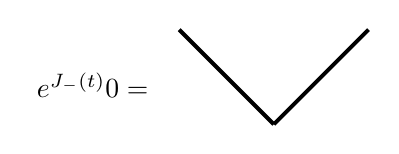
\begin{tikzpicture}
    \node at (-2.3,.5) {\(e^{\bm{J}_-(\bm{t})} \ket{\bm{0}} =\)};
    \draw[line width=0.5mm][rotate=45]   (0,0) -- (0,1.7);
    \draw[line width=0.5mm][rotate=45]   (0,0) -- (1.7,0);
    \end{tikzpicture}
    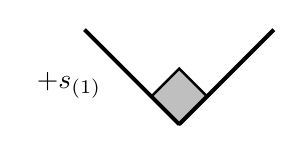
\begin{tikzpicture}
    \node at (-1.4,.5) {\(+ s_{(1)}\)};
    \draw [line width=0.3mm][rotate=45][fill=lightgray]  (0,0) rectangle (.5,.5);
    \draw[line width=0.5mm][rotate=45]   (0,0) -- (0,1.7);
    \draw[line width=0.5mm][rotate=45]   (0,0) -- (1.7,0);
    \end{tikzpicture}		
    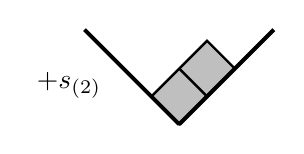
\begin{tikzpicture}
    \node at (-1.4,.5) {\(+ s_{(2)}\)};
    \draw [line width=0.3mm][rotate=45][fill=lightgray] (0,0) rectangle (1,.5);
    \draw[line width=0.3mm][rotate=45]   (0.5,0) -- (0.5,.5);
    \draw[line width=0.5mm][rotate=45]   (0,0) -- (0,1.7);
    \draw[line width=0.5mm][rotate=45]   (0,0) -- (1.7,0);
    \end{tikzpicture}		
    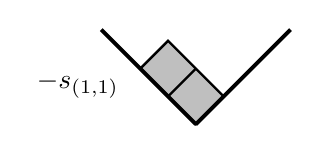
\begin{tikzpicture}
    \node at (-1.5,.5) {\(- s_{(1,1)}\)};
    \draw [line width=0.3mm][rotate=45][fill=lightgray] (0,0) rectangle (.5,1);
    \draw[line width=0.3mm][rotate=45]   (0,.5) -- (.5,.5);
    \draw[line width=0.5mm][rotate=45]   (0,0) -- (0,1.7);
    \draw[line width=0.5mm][rotate=45]   (0,0) -- (1.7,0);
    \end{tikzpicture}
    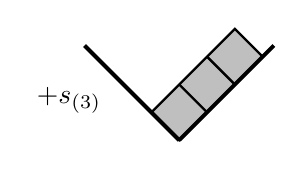
\begin{tikzpicture}
    \node at (-1.4,.5) {\(+ s_{(3)}\)};
    \draw [line width=0.3mm][rotate=45][fill=lightgray] (0,0) rectangle (1.5,0.5);
    \draw[line width=0.3mm][rotate=45]   (.5,0) -- (.5,.5);
    \draw[line width=0.3mm][rotate=45]   (1,0) -- (1,.5);
    \draw[line width=0.5mm][rotate=45]   (0,0) -- (0,1.7);
    \draw[line width=0.5mm][rotate=45]   (0,0) -- (1.7,0);
    \end{tikzpicture}
    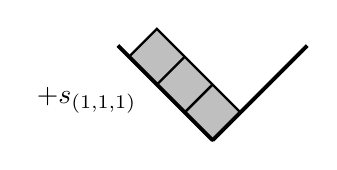
\begin{tikzpicture}
    \node at (-1.6,.5) {\(+ s_{(1,1,1)}\)};
    \draw [line width=0.3mm][rotate=45][fill=lightgray] (0,0) rectangle (.5,1.5);
    \draw[line width=0.3mm][rotate=45]   (0,.5) -- (.5,.5);
    \draw[line width=0.3mm][rotate=45]   (0,1) -- (.5,1);
    \draw[line width=0.5mm][rotate=45]   (0,0) -- (0,1.7);
    \draw[line width=0.5mm][rotate=45]   (0,0) -- (1.7,0);
    \end{tikzpicture}
    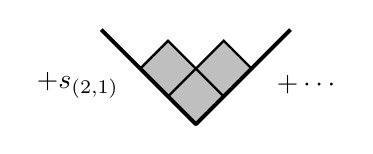
\begin{tikzpicture}
    \node at (-1.5,.5) {\(+ s_{(2,1)}\)};
    \draw [line width=0.3mm][rotate=45][fill=lightgray] (0,0) rectangle (.5,1);
    \draw [line width=0.3mm][rotate=45][fill=lightgray] (0,0) rectangle (1,.5);	
    \draw[line width=0.3mm][rotate=45]   (.5,0) -- (.5,.5);		
    \draw[line width=0.5mm][rotate=45]   (0,0) -- (0,1.7);
    \draw[line width=0.5mm][rotate=45]   (0,0) -- (1.7,0);
    \node at (1.4,.5) {\(+ \cdots\)};
    \end{tikzpicture}							
\end{center}
where the coefficients are
\begin{equation}
s_{(1)}=t_{-1}\; , \quad s_{(2)}=\frac{1}{2}t_{-1}^2 + t_{-2} \; ,\quad s_{(1,1)}
=\frac{1}{2}t_{-1}^2- t_{-2}\; ,\quad  \dots
\end{equation}

The Miwa coordinates are given by \(t_j = \frac{1}{j}\sum_{a = 1}^j
x_a^m\) where \(\bm{x} = (x_1, x_2, \dots, x_m)\) is a set of \(m\)
variables. If we write these Schur functions in terms of \(\bm{x}\),
these functions become symmetric polynomials, and we call them
\emph{Schur polynomials}. In terms of these coordinates, the Schur
polynomials are characters of the \(\lambda\) representations
evaluated at the diagonal matrix \(\mathrm{diag}(x_1, x_2, \dots,
x_m)\). In any case, in the text we use both terminologies as
synonyms.

%%%%%%%%%%%%%%%%%%%%%%%
%%%%%%%%%%%%%%%%%%%%%%%

\subsection{Fermion-Boson correspondence}

The fermion boson correspondence is a relation between basis of
Hilbert space~\cite{Cordes:1994fc, Marino:2005sj}. Let start this
definition with some basic facts. The complete homogeneous symmetric
polynomials are defined by
\begin{equation}
  \label{eq:com-hom-sym-pol}
\exp\left(\sum_{k\geq 1} T_k z^k\right): = \sum_{k\geq 0} h_k(\bm{T}) z^k \; ,
\end{equation}
with \(h_0=1\) and we also define \(h_{-k}=0\  \forall\ k>0\). Explicitly we have 
\begin{equation}
  h_k(\bm{T}) = \sum_{k_1+2k_2 +\dots = k}\frac{T_1^{k_1}}{k_1!} \frac{T_2^{k_2}}{k_2!}\cdots
  \; .
\end{equation}	

We can use this polynomials to express the \emph{coherent state}
\begin{equation}
\begin{split}
  \ket{\mathcal{T}}& = \exp\left( \sum_{n\geq 1} t_{n} J_{-n}\right) \ket{\bm{0}} = 
  \exp\left.\left(\sum_{n\geq 1} T_n z^n\right)\right|_{z=1}  \ket{\bm{0}} \\
& = \sum_{k\geq 0} \sum_{k_1+2k_2+\cdots = k}\frac{t_{1}^{k_1}}{k_1!}
\frac{t_{2}^{k_2}}{k_2!}\cdots \ket{k_1, k_2, k_3\dots}
\end{split}
\end{equation}
where we have used that \(T_k \equiv t_k J_{-k}\), \(\bm{t}_- = (t_1,
t_2 \dots)\) , \(\vec{k} = (k_1, \dots, k_r)\) and \(\sum_j j k_j =
|\lambda|\).  One should observe that in contrast with our previous
definition, the parameters \(\bm{t}_-\) have been changed to
\(\bm{t}_+\equiv \bm{t}\). Since there is no intrinsic meaning in those objects,
this transformation is just a relabeling.

Using the expansion of \(\ket{\vec{k}}\) in terms of characters
coefficients, we can write the explicit expression for the Schur as
\begin{equation}
\begin{split}
  \ket{\mathcal{T}}& = \sum_{\lambda} s_\lambda(\bm{t})\ket{\lambda} \\
    & = \sum_\lambda\left( \sum_{k\geq 0} \sum_{k_1+2k_2+\cdots = k}\frac{t_{1}^{k_1}}{k_1!}
    \frac{t_{2}^{k_2}}{k_2!}\cdots \chi_\lambda [C(\vec{k})] \right) \ket{\lambda}
\end{split}
\end{equation}
This formula is very hard to calculate explicily, but it is useful to know that
if we change the coefficients \(\chi_\lambda\), we have a new type of fermion boson
correspondence. 

If we now identify \(t_{j} \equiv \frac{1}{j}P_j(x)\), we can
write all expressions in terms of the coordinates \(\vec{x}\). And we
conclude that
\begin{equation}
\langle \mathcal{T}| \vec{k} \rangle= \langle \vec{k} |\mathcal{T}\rangle = P_{\vec{k}}(x)\; .
\end{equation}

Moreover, we have seen that Schur polynomials are defined as
\(s_{\lambda}(t)=\langle \mathcal{T}| \lambda \rangle\), and since
Schur and Newton polynomials are related by the Frobenius formula, it
is easy to see that there is a relation between the fermionic and
bosonic states. This relation is the Fermion-Boson correspondence.
